\begin{figure}[!t]
%%%
\begin{subfigure}{.24\textwidth}
%%%
    \resizebox{\linewidth}{!}{%

    \begin{minipage}[t]{.99\linewidth}
    \centering
    \strut\vspace*{-9mm}\newline
    
        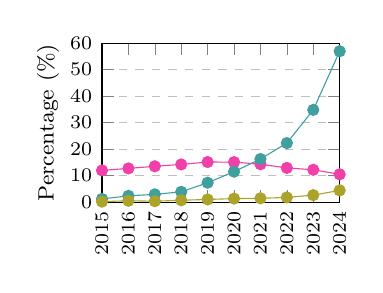
\begin{tikzpicture}
            \begin{axis}[
                /pgf/number format/1000 sep={},
                %xlabel={Publishing year},
                ylabel={Percentage (\%)},
                ylabel style={yshift=-1mm},
                %xmin=2000, xmax=2024,
                xmin=2015, xmax=2024,
                ymin=0, ymax=60,
                %xtick={2000,2005,2010,2015,2020,2025},
                xtick={2015,2016,2017,2018,2019,2020,2021,2022,2023,2024,2025},
                ytick={60,50,40,30,20,10,0},
                height=3.6cm,
                width=4.6cm,
                legend pos=north west,
                ymajorgrids=true,
                grid style=dashed,
                title style={yshift=-3mm},
                xlabel style = {font=\footnotesize},
                ylabel style = {font=\footnotesize},
                xticklabel style = {font=\scriptsize, rotate=90},
                yticklabel style = {font=\scriptsize},
                legend style={font=\scriptsize},
                % line width=0.2mm,
                % title={x}
            ]

            \addplot[
                color=magenta!75!white,
                mark=*,
                ]
                coordinates {
                %(2000,10.18)(2001,19.55)(2002,13.43)(2003,14.99)(2004,9.59)(2005,18.76)(2006,12.87)(2007,16.80)(2008,15.71)(2009,14.49)(2010,15.21)(2011,15.27)(2012,15.37)(2013,13.57)(2014,14.69)
                (2015,11.96)(2016,12.71)(2017,13.51)(2018,14.21)(2019,15.12)(2020,15.09)(2021,14.29)(2022,12.90)(2023,12.20)(2024,10.48)
                };
            %\addlegendentry{MT}

            \addplot[
                color=teal!75!white,
                mark=*,
                ]
                coordinates {
                %(2000,0.92)(2001,1.71)(2002,0.86)(2003,1.53)(2004,1.02)(2005,2.16)(2006,1.91)(2007,1.62)(2008,2.23)(2009,1.58)(2010,1.34)(2011,2.01)(2012,1.93)(2013,2.09)(2014,2.10)
                (2015,1.19)(2016,2.36)(2017,2.91)(2018,3.86)(2019,7.31)(2020,11.48)(2021,16.25)(2022,22.28)(2023,34.81)(2024,56.94)
                };
            %\addlegendentry{LM}

            \addplot[
                color=olive!75!white,
                mark=*,
                ]
                coordinates {
                %(2000,0.08)(2001,0.26)(2002,0.17)(2003,0.27)(2004,0.22)(2005,0.58)(2006,0.43)(2007,0.52)(2008,0.88)(2009,0.14)(2010,0.40)(2011,1.01)(2012,0.49)(2013,0.62)(2014,0.80)
                (2015,0.17)(2016,0.49)(2017,0.33)(2018,0.69)(2019,0.99)(2020,1.31)(2021,1.43)(2022,1.76)(2023,2.61)(2024,4.41)
                };
            %\addlegendentry{MT + LM}
            \end{axis}
        \end{tikzpicture}
        %\\

        \end{minipage}
}%
	%\caption{MT (red), LM (blue), MT+LM (green).}
	%\label{fig:trend}

%%%
\end{subfigure}%
\hfill
\begin{subfigure}{.24\textwidth}
%%%

    \resizebox{\linewidth}{!}{%

    \begin{minipage}[t]{.99\linewidth}
    \centering
    \strut\vspace*{-9mm}\newline
    
        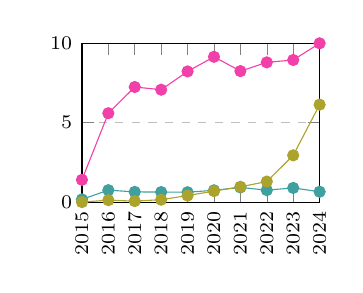
\begin{tikzpicture}
            \begin{axis}[
                /pgf/number format/1000 sep={},
                %xlabel={Publishing year},
                ylabel={\textcolor{white}{\%}},
                ylabel style={yshift=-3mm},
                %xmin=2000, xmax=2024,
                xmin=2015, xmax=2024,
                ymin=0, ymax=10,
                %xtick={2000,2005,2010,2015,2020,2025},
                xtick={2015,2016,2017,2018,2019,2020,2021,2022,2023,2024,2025},
                ytick={10,5,0},
                height=3.6cm,
                width=4.6cm,
                legend pos=north west,
                ymajorgrids=true,
                grid style=dashed,
                title style={yshift=-3mm},
                xlabel style = {font=\footnotesize},
                ylabel style = {font=\footnotesize},
                xticklabel style = {font=\scriptsize, rotate=90},
                yticklabel style = {font=\scriptsize},
                legend style={font=\scriptsize},
                % line width=0.2mm,
                % title={x}
            ]

            \addplot[
                color=magenta!75!white,
                mark=*,
                ]
                coordinates {
                %(2000,1.50)(2001,2.23)(2002,1.88)(2003,1.80)(2004,1.94)(2005,1.41)(2006,4.98)(2007,1.30)(2008,4.88)(2009,0.98)(2010,4.80)(2011,1.51)(2012,5.31)(2013,1.65)(2014,4.55)
                (2015,1.40)(2016,5.59)(2017,7.24)(2018,7.07)(2019,8.22)(2020,9.14)(2021,8.24)(2022,8.79)(2023,8.94)(2024,9.99)
                };
            %\addlegendentry{Users}

            \addplot[
                color=teal!75!white,
                mark=*,
                ]
                coordinates {
                %(2000,1.00)(2001,1.71)(2002,0.77)(2003,0.81)(2004,0.75)(2005,0.75)(2006,0.72)(2007,0.26)(2008,0.74)(2009,0.14)(2010,0.57)(2011,0.59)(2012,1.20)(2013,0.15)(2014,0.91)
                (2015,0.17)(2016,0.75)(2017,0.64)(2018,0.63)(2019,0.62)(2020,0.74)(2021,0.92)(2022,0.75)(2023,0.89)(2024,0.65)
                };
            %\addlegendentry{MT + user}

            \addplot[
                color=olive!75!white,
                mark=*,
                ]
                coordinates {
                %(2000,0)(2001,0)(2002,0)(2003,0)(2004,0)(2005,0)(2006,0.05)(2007,0)(2008,0)(2009,0)(2010,0)(2011,0)(2012,0)(2013,0)(2014,0.11)
                (2015,0)(2016,0.12)(2017,0.06)(2018,0.15)(2019,0.41)(2020,0.69)(2021,0.96)(2022,1.29)(2023,2.94)(2024,6.13)
                };
            %\addlegendentry{LM + user}
            \end{axis}
        \end{tikzpicture}
        %\\

        \end{minipage}
}%
	%\caption{Users (red), MT and users (blue), LM + users (green).}
	%\label{fig:trend2}
%%%
\end{subfigure}%
%%%

\caption{Trend of interest in \emph{machine translation} (\textsc{mt}), \emph{language models} (\textsc{lm}), \emph{users} (\textsc{u}), and combinations thereof in the ACL community over the last 10 years. \textbf{Left}:~\textcolor{magenta}{\textsc{\textbf{mt}}}, \textcolor{teal}{\textsc{\textbf{lm}}}, \textcolor{olive}{\textsc{\textbf{mt+lm}}}. \textbf{Right}:~\textcolor{magenta}{\textsc{\textbf{u}}}, \textcolor{teal}{\textsc{\textbf{mt+u}}}, \textcolor{olive}{\textsc{\textbf{lm+u}}}.\footnotemark}
\label{fig:trend-overview}

\end{figure}